% ========== VILDSVIN ==========
\begin{frame}{%
  \begin{minipage}[c]{0.30\textwidth}
    Vildsvin
  \end{minipage}%
  \hfill
  \begin{minipage}[c]{0.45\textwidth}
    \footnotesize
    \textbf{Jagttid:} Orne: 1.\ sep.--31.\ jan.\\
    So og gris: 1.\ okt.--31.\ jan.
  \end{minipage}%
  \hfill
  \begin{minipage}[c]{0.15\textwidth}
    \noindent\raggedleft
    
\includegraphics[width=0.5cm, height=0.5cm, keepaspectratio]{Billeder/Ikoner/star.png}%
    \hspace{0.2em}%
    
\includegraphics[width=0.5cm, height=0.5cm, keepaspectratio]{Billeder/Ikoner/star.png}
  \end{minipage}%
}
  \vspace{0.25em}
  \begin{columns}[T]
    \column{0.45\textwidth}
    \setlength{\parskip}{0.4em}
    \tiny
    \RaggedRight
    \textbf{\textit{Sus scrofa}} – langt, kegleformet hoved og kompakt krop med kraftig, børstet pels. Ornen har synlige hjørnetænder. \par
    \textbf{Benævnes:}\\
    \quad – Han: Orne \\
    \quad – Hun: So \\
    \quad – Unge: Gris \par
    \textbf{Udseende:}\\
    \quad – Ligner en gris \\
    \quad – Kraftig, strid pels \\
    \quad – Kompakt krop \par
    \textbf{Levesteder:} Findes i alle landskabstyper. Meget sky og nataktiv. \par
    \textbf{Føde:} Altædende, bl.a. planter, rødder, orme og ådsler. \par
    \textbf{Udbredelse:} Strejfende individer i Sydjylland. \par
    %\textbf{Forplantning:}\\
    %\quad – \textbf{Kønsmoden:} Ca. 1 år \\
    %\quad – \textbf{Mono/polygam:} Polygam \\
    %\quad – \textbf{Bestandsomsætning:} Hurtig \\
    %\quad – \textbf{Kuld:} 4--8 grise
    \column{0.52\textwidth}
    \centering
    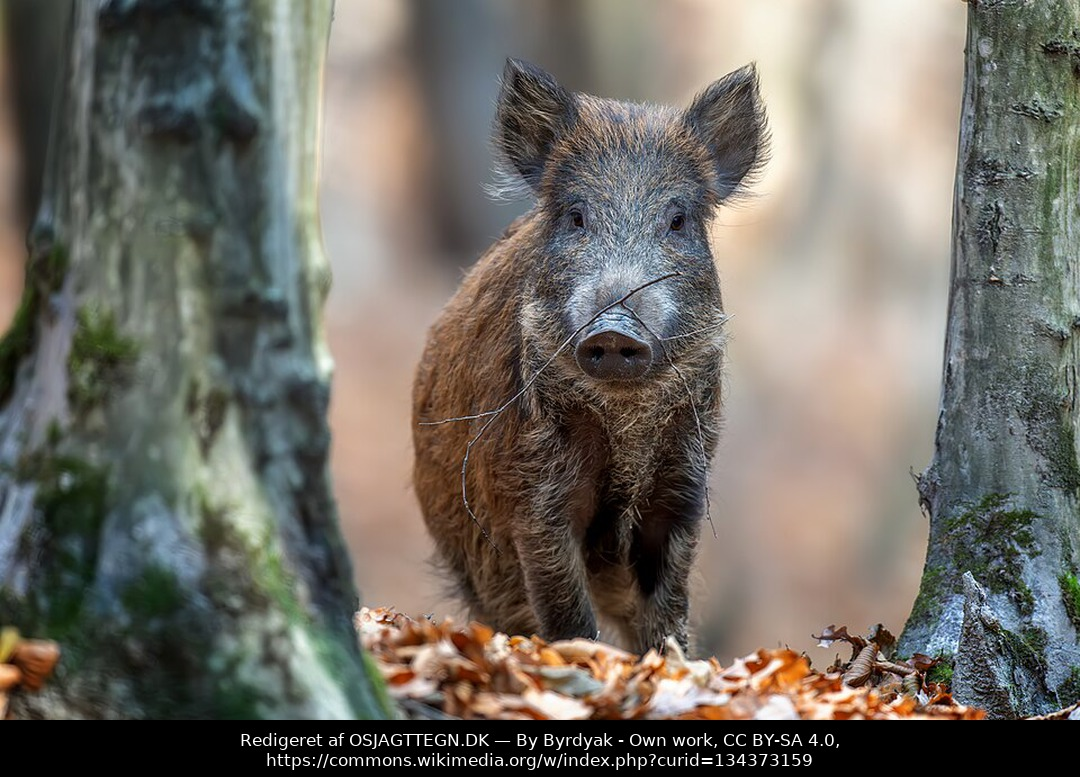
\includegraphics[width=\linewidth, height=7.2cm, keepaspectratio]{Billeder/Dyr/Pattedyr/hovdyr/vildsvin/vildsvin-01.jpg}
  \end{columns}
\end{frame}